\documentclass[conference,a4paper,10pt,oneside,final]{tfmpd}
\usepackage[latin1]{inputenc}   % caracteres especiales (acentos, eñes)

\usepackage[spanish]{babel}     % varias definiciones para el español
\usepackage{graphicx}           % inserción de graficos

% Paquetes adicionales de símbolos matemáticos
\usepackage{amsmath,amssymb,amsfonts,latexsym,cancel} 

\usepackage{booktabs} % Opciones adicionales para el entorno tabular
\usepackage{longtable} % Para tablas de más de una página
\usepackage{multirow}

\usepackage{listings} %Para escribir códigos
\lstset{%language=XML,
	basicstyle=\footnotesize,
	numbers=left,
 	stepnumber=1,
	numbersep=3pt,
	showspaces=false,               % show spaces adding particular underscores
  	showstringspaces=false,         % underline spaces within strings
  	frame=lines,                   % adds a frame around the code
	tabsize=4,                      
  	captionpos=b,                   % sets the caption-position to bottom
  	breaklines=true,                % sets automatic line breaking
  	keywords={repetir,para,hasta,devolver,evaluar,seleccionar,cruzarymutar,mientras,fin_mientras,inicializar},
}
%---

\usepackage{pstricks}

\begin{document}

\title{Búsqueda del camino óptimo entre dos ciudades mediante el algoritmo del sistema de hormigas: Trabajo Final de Inteligencia Computacional}

\author{Marco A. Pereyra,
        Gaspar E. Oberti y 
        Darién J. Ramírez \\
\textit{Trabajo práctico final de ``Inteligencia Computacional'', II-FICH-UNL.}}

\markboth{INTELIGENCIA COMPUTACIONAL: TRABAJO FINAL}{}

\maketitle

\begin{abstract}
En este artículo se propone un algoritmo para determinar el camino óptimo entre dos ciudades de la provincia de Santa Fe a través del algoritmo de \textit{sistema de hormigas}. El camino óptimo no está basado sólo en la distancia, éste dependerá de más factores tales como peajes en las rutas, niveles de tráfico, etc. Esos factores serán representados a través de matrices simétricas de relación entre ciudades y su influencia en la elección del camino estará aplicada sobre los depósitos de feromonas. Los resultados obtenidos serán comparados con otros métodos de elección de caminos.
\end{abstract}

\begin{keywords}
sistema de hormigas, algoritmo genético, costo uniforme, camino óptimo, costo de camino.
\end{keywords}

\section{Introducción}

\PARstart{E}{l} problema de encontrar el camino óptimo entre dos ciudades consiste en establecer un punto de partida y un punto de destino, luego hallar entre todos los posibles caminos el óptimo. Esto es, encontrar un camino que satisfaga ciertos requerimientos deseados y lo haga de la mejor manera posible. Este problema en particular está normalmente asociado a la distancia de ir de una ciudad a otra de modo que el camino óptimo es aquel que minimice la distancia. Pero no necesariamente es siempre así, se pueden solicitar otras características que ponderen a los posibles caminos como son los puestos de peaje en las rutas, los niveles de tráfico, la disponibilidad hotelera, entre otras.
Existen muchos métodos para poder realizar esta tarea. Algunos más rápidos que otros, algunos más efectivos que otros, algunos con menos costo computacional que otros. En el presente trabajo utilizaremos el algoritmo de \textit{Sistema de Hormigas} (AS) para realizar esta tarea porque lo consideramos una buena opción para atacar este problema dentro de los métodos que conocemos de la inteligencia computacional.
Los sistemas de hormigas tienen la capacidad para adaptarse, cooperar y moverse  inteligentemente de un sitio a otro. Las propiedades inherentes de los sistemas de hormigas incluyen la escalabilidad, la posibilidad de descubrir nuevas vías y soluciones, y la inteligencia, la baja complejidad de las interacciones locales y la comunicación a través del sistema. En general, las hormigas reales son capaces de hallar el camino más corto entre una fuente de alimento y su nido segregando 
sustancias químicas llamadas feromonas. Las hormigas hacen uso de feromonas marcadoras de pistas para indicar el mejor camino a las siguientes hormigas. Este comportamiento de las hormigas reales ha inspirado los sistemas de hormigas, algoritmos en los 
que un grupo de hormigas artificiales transitan los caminos y cooperan para encontrar la solución de un problema intercambiando información mediante las feromonas depositadas en las rutas. A continuación se comentarán algunos detalles de la implementación utilizada.

\section{Implementación}

Para el presente trabajo se utilizó el algoritmo \ref{fig:AS} de sistema de hormigas al cual se le realizaron modificaciones para tener en cuenta no solo el costo de viaje por medio de la distancia sino también para considerar otras características en la búsqueda del camino óptimo.
En primer lugar, a tiempo cero, se inicializa la matriz de feromonas con datos de distribución uniforme aleatoria. Las hormigas son ubicadas inicialmente en la ciudad de origen, aquella de donde se parte, para que después se encarguen de recorrer los caminos posibles a la ciudad destino y determinar de manera porcentual cuál es el camino que arroja el mejor resultado dependiendo de las características evaluadas. A medida que una hormiga se desplaza de ciudad en ciudad se irán eliminando de la lista de posibles caminos las aristas correspondientes a las rutas ya visitadas. De este modo, se ahorra el tener que eliminar los bucles de un camino encontrado a la ciudad destino. Una característica interesante de este algoritmo es la presencia de la variable $\eta_{ij}^{\beta}(t)$, inversa de la distancia entre nodos, que representa el deseo de la hormiga de moverse en una dirección en particular y permite que el algoritmo evalúe no solo las feromonas si no también las otras características.

\begin{figure}[!h]
\begin{lstlisting}[mathescape=true]
t$=0$,$\sigma_{ij}(t)\leftarrow U(0,\sigma_{0})$
Ubicar $N$ hormigas en el nodo origen
repetir
	para cada hormiga $k=1,2,...,N$
		p$^{k}(t)=\varnothing$
		repetir
			$\bullet$ seleccionar el próximo nodo según probabilidad $p_{ij}^{k}(t)=\begin{cases}
\frac{\sigma_{ij}^{\alpha}(t)\eta_{ij}^{\beta}(t)}{\sum_{\forall u\in N_{i}^{k}}\sigma_{ui}^{\alpha}(t)\eta_{ij}^{\beta}(t)} & ;j\in N_{i}^{k} \\
0;&; e.o.c.
\end{cases}$
			$\bullet$ agregar un paso $(i,j)$ al camino $p^{k}(t)$
		hasta alcanzar el destino
		calcular la longitud del camino encontrado $f(p^{k}(t))$
	para cada conexión $(i,j)$
		$\bullet$ reducir por evaporación la cantidad de feromonas: $\sigma_{ij}(t)\leftarrow(1-\rho)\sigma_{ij}(t)$
		$\bullet$ depositar feromonas proporcionalmente a la bondad de la solución $\Delta\sigma_{ij}^{k}(t)=
\begin{cases} 
\frac{Q}{f(p^{k}(t))} & global \\
Q & uniforme \\
\frac{Q}{d_{ij}} & local
\end{cases}$$\sigma_{ij}(t+1)=\sigma_{ij}(t)+\sum_{\forall k/(i,j)\in p^{k}(t)}\Delta\sigma_{ij}^{k}(t)$
hasta que todas las hormigas sigan el mismo camino
devolver el mejor camino
\end{lstlisting}
\caption{Algoritmo: Sistema de Hormigas}
\label{fig:AS}
\end{figure}


La función $f(p^{k}(t))$ representa el costo del camino encontrado. Como no sólo se tiene en cuenta la distancia si no también otros factores, habrá un costo de camino para cada una de las características evaluadas. La evaporación de las feromonas representa el comportamiento de las mismas que se da en la naturaleza. La velocidad con la cual se produce la evaporación se encuentra regulada por un parámetro $\rho$. Cuanto más grande sea su valor, mayor será el nivel de disipación feromonal.

A la hora de realizar el depósito de feromonas se utiliza el depósito global. Este fue elegido tras realizar sucesivas pruebas con los tres métodos de depósito de feromonas ya que se encontraron mejores resultados con el método electo. El valor de la constante Q se fijó en 1. En esta parte es donde se tienen en cuenta las distintas características para actualizar los valores de la feromonas:

\begin{align*}
\frac{Q}{f_{1}(p^{k}(t))}+\frac{Q}{f_{2}(p^{k}(t))}+\cdots+\frac{Q}{f_{n}(p^{k}(t))}
\end{align*}

Esto permite que las distintas características hagan su aporte en la actualización de los valores de la matriz de feromonas. Estas funciones de costo están directamente relacionadas con las matrices de relación entre ciudades.

\section{Matrices de relación}

Las matrices de relación entre ciudades contienen los costos de las diferentes características de evaluación de caminos. Para este trabajo en particular se definieron cuatro matrices: distancias, peajes, tráfico y hospedaje.
A nivel general estas matrices contienen información correspondiente a las aristas de un grafo, es decir, el costo representado en la celda $i,j$ de las matrices representa el costo de ir de la ciudad $A$ a la ciudad $B$ y como son simétricas la celda $j,i$ representa el costo de ir de la ciudad $B$ a la ciudad $A$.

Existen ciudades que no tienen una conexión física entre ellas. En estos casos la celda $i,j$ de las matrices tienen un valor no válido de costo. Esto es para que las hormigas no puedan optar por tomar un camino inexistente entre ciudades y se adapten a la estructura del problema planteado y representado por las matrices de relación. Por otra parte, la diagonal de las matrices son nulas puesto que la distancia de una ciudad a si misma es nula. Aun así dado el funcionamiento del algoritmo, si se está parado en una ciudad, no se elegirá esa misma ciudad como posible camino.

A continuación se muestran ejemplos de matrices de relación de $3\times3$ para visualizar mejor su estructura:

\begin{figure}[!h]
\begin{align*}
D = \bordermatrix{
~                 & \textit{Santa Fe} & \textit{Esperanza} & \textit{Recreo} \cr
\textit{Santa Fe} & 0                 & -1                  & 17 			  \cr
\textit{Esperanza}& -1                & 0                   & 22              \cr
\textit{Recreo}   & 17                & 22                  & 0}
\end{align*}
\caption{Matriz de distancias}
\label{fig:MD}
\end{figure}

La fila 1 de $D$ (Figura \ref{fig:MD}) se lee como:

\begin{itemize}
\item Santa Fe tiene distancia nula consigo misma.
\item No hay una ruta que conecte Santa Fe con Esperanza.
\item Santa Fe tiene una ruta que la conecta a Recreo cuya distancia es de 17 km. También es posible verlo como que el costo para viajar desde Santa Fe a Recreo o desde Recreo a Santa Fe es 17.
\end{itemize}

\begin{figure}[!h]
\begin{align*}
P = \bordermatrix{
~                 & \textit{Santa Fe} & \textit{Esperanza} & \textit{Recreo} \cr
\textit{Santa Fe} & 0                 & -1                  & 0 			  \cr
\textit{Esperanza}& -1                & 0                   & 2               \cr
\textit{Recreo}   & 0                 & 2                   & 0}
\end{align*}
\caption{Matriz de peajes}
\label{fig:MP}
\end{figure}

Los posibles valores para la matriz de peajes (Figura \ref{fig:MP}) (sin contar la diagonal y las posiciones inválidas) son los números $0,1,\dots,5$. El cero indica no hay una estación de peaje en la ruta que une esas dos ciudades determinadas. Los números restantes no indican el precio del peaje si no un indicador de costo.

\begin{itemize}
\item \textbf{1}: Muy económico.
\item \textbf{2}: Económico.
\item \textbf{3}: Intermedio.
\item \textbf{4}: Costoso.
\item \textbf{5}: Muy costoso.
\end{itemize}

\begin{figure}[!h]
\begin{align*}
T = \bordermatrix{
~                 & \textit{Santa Fe} & \textit{Esperanza} & \textit{Recreo} \cr
\textit{Santa Fe} & 0                 & -1                  & 27 			  \cr
\textit{Esperanza}& -1                & 0                   & 27              \cr
\textit{Recreo}   & 27                & 27                  & 0}
\end{align*}
\caption{Matriz de tránsito}
\label{fig:MT}
\end{figure}

Los valores en la matriz de tránsito (Figura \ref{fig:MT}) indican una cantidad de minutos aproximada en la que es posible recorrer la distancia teniendo en cuenta el tráfico habitual de la ruta.

\begin{figure}[!h]
\begin{align*}
H = \bordermatrix{
~                 & \textit{Santa Fe} & \textit{Esperanza} & \textit{Recreo} \cr
\textit{Santa Fe} & 0                 & -1                  & 9 			  \cr
\textit{Esperanza}& -1                & 0                   & 1               \cr
\textit{Recreo}   & 9                 & 1                   & 0}
\end{align*}
\caption{Matriz de hospedaje}
\label{fig:MH}
\end{figure}

Los valores en la matriz de hospedaje (Figura \ref{fig:MH}) indican la cantidad de lugares con alojamiento que se encuentran en el camino entre las dos ciudades.

Todas las matrices de relación tienen en común que son simétricas, la diagonal es nula y que las posiciones inválidas se corresponden, el resto de las celdas son valores propios del tipo de matriz en cuestión.

Entonces el deseo de moverse de la hormiga ya no será sólo la inversa de la distancia si no que será la suma de las inversas de cada característica aplicada. Lo mismo ocurre a la hora de depositar feromonas en base a la bondad de la solución.

\begin{align*}
\sigma_{ij}(t+1)=
\sigma_{ij}(t)+\sum_{\forall k/(i,j)\in p^{k}(t)}\Delta\sigma_{ij}^{k}(t)
\end{align*}

donde \\

$
\Delta\sigma_{ij}^{k}(t)
=\frac{Q}{f_{D}(p^{k}(t))}
+\frac{Q}{f_{P}(p^{k}(t))}
+\frac{Q}{f_{T}(p^{k}(t))}
+\frac{Q}{f_{H}(p^{k}(t))}
$ \\

Como se puede notar las proporciones de éstas matrices son muy diferentes entre si. Por lo tanto, para poder realizar una comparación válida entre ellas a la hora de hacer sus aportes a la matriz de feronomas, serán normalizadas. Para esto se toma el valor máximo de cada matriz y se las divide por dicho valor obteniendo así matrices normalizadas con valores que van entre cero y uno.

\section{Algoritmo genético}

Además del algoritmo de hormigas también se ha desarrollado un algoritmo genético para encontrar el camino óptimo entre dos ciudades de modo de poder hacer una comparación entre los resultados arrojados por ellos.

\begin{figure}[!h]
\begin{lstlisting}[mathescape=true]
inicializar(población)
mejor_fitness=evaluar(población)
mientras (mejor_fitness < fitness_requerido)
	selección=seleccionar(población)
	población=cruzarymutar(selección)
	mejor_fitness=evaluar(población)
fin_mientras
\end{lstlisting}
\caption{Algoritmo genético}
\label{fig:AG}
\end{figure}

Para un ejemplo donde se consta de 7 ciudades el material genético se encuentra codificado de la siguiente manera:

\begin{center}
\resizebox{\linewidth}{!}{
\begin{tabular}{cccccccccc}
fenotipo & 5   & $\rightarrow$ & 1   & $\rightarrow$ & 4   & $\rightarrow$ & 2   & $\rightarrow$ & 3 \\
genotipo & 101 & $\rightarrow$ & 001 & $\rightarrow$ & 100 & $\rightarrow$ & 010 &$\rightarrow$ & 011
\end{tabular}}
\end{center}

Cada número en el fenotipo está asociado a una ciudad. Su codificación genética consiste en la representación binaria del número que se asocia a la ciudad. El primer elemento representa la ciudad de origen y el último elemento representa la ciudad de destino. Los elementos intermedios representan las ciudades por las que hay que pasar para llegar del origen al destino.

Para determinar el \textit{fitness} se convierte el genotipo a fenotipo (Tabla \ref{table:gtof}), se mide y suma la distancia entre la ciudades y finalmente se calcula la inversa del valor del camino.

\begin{table}[!h]
\begin{tabular}[c]{|c|c|c|c|c|c|c|c|c|} \hline
Fenotipo & 0   & 1   & 2   & 3   & 4   & 5   & 6   & 7   \\ \hline
Genotipo & 000 & 001 & 010 & 011 & 100 & 101 & 110 & 111 \\ \hline
\end{tabular}
\caption{Conversión de genotipo a fenotipo.}
\label{table:gtof}
\end{table}

El método de selección usado es el método de ventanas. Se ordenan los individuos según su \textit{fitness} (de mejor a peor) y se van definiendo ventanas cada vez más pequeñas sacando un individuo (progenitor) al azar para cada una. Las ventanas van dejando de lado a los peores individuos.

Para realizar las mutaciones no se tocan los bits más significativos correspondientes al origen ni los menos significativos correspondientes al destino, se toman los bits de los destinos intermedios al azar. Existe una probabilidad $p$ de que exista una mutación. De los bits del destino intermedio seleccionado se modifica un bit al azar y se cambia su valor (cero por uno o uno por cero). Tras la mutación se debe comprobar si la ciudad generada es válida revisando las conexiones con el nodo anterior y el siguiente. Si no lo es, se vuelve a repetir el proceso de mutación hasta generar una válida.

Para realizar la cruza se elige una ciudad al azar entre las intermedias como punto de cruza. Entonces el material genético anterior a ese punto de cruza de uno de los padres se combina con el material genético del otro padre a partir e incluyendo el valor del punto de cruza. Si el camino no es válido se vuelve a repetir la cruza hasta obtener uno válido.

\begin{align*}
{\red 101 001 \stackrel{pc}{100} 010 011} &\rightarrow 
{\red 101 001} 001 010 011 \\
101 \stackrel{pc}{001} 010 011 &\rightarrow
101 {\red 100 010 011}
\end{align*}

El tamaño de la población es constante pero el tamaño de los genotipos es variable puesto que depende de la longitud del camino. El método de remplazo utilizado durante la reproducción es el elitismo que implica agregar a la siguiente generación al individuo con mejor \textit{fitness} de la generación actual.

\section{Método de búsqueda costo uniforme}

Éste método ha sido implementado, así como el algoritmo genético, para realizar comparaciones de resultados con el algoritmo de las hormigas.

En el método de búsqueda costo uniforme todos los nodos de profundidad $d$ en el árbol de búsqueda se expanden antes que los nodos de profundidad $d+1$. Además esa expansión es siempre primero para el nodo de menor costo, medido por una función que evalúa el \textit{costo del camino} $g(n)$. Su implementación es una lista ordenada de menor a mayor costo. Cuando se verifican ciertas condiciones se garantiza que la primer solución que se encuentra es la de mínimo costo. La restricción es que el costo de un camino nunca debe decrecer al avanzar en su desarrollo.

\section{Resultados}

En la tabla \ref{table:tab1} se muestran los tiempos de ejecución en segundos obtenidos con los tres algoritmos planteados para distinta cantidad de ciudades. El algoritmo de hormigas fue ejecutado con 7 hormigas en cada caso y el coeficiente de evaporación $\rho$ fue fijado en 0,8. Al algoritmo genético se le estableció una población de 8 individuos en todos los casos y fue ejecutado hasta alcanzar las 10 generaciones. Los tiempos se corresponden a una sola ejecución del algoritmo y sólo se ha tenido en cuenta la distancia.

\begin{table}[!h]
\begin{center}
\begin{tabular}[c]{cccc} \toprule
Dimensión de la matriz & Hormigas & Genético & Costo Uniforme \\ \midrule
$7\times7$    & 0.36  & 2.72 & 0.32     \\
$10\times10$  & 1.13  & 5.31 & 3.72     \\
$15\times15$  & 6.45  & 9.71 & 35.33    \\
$20\times20$  & 13.11 & 18.7 & 243.42   \\ \bottomrule    
\end{tabular}
\end{center}
\caption{Comparativa de tiempos de ejecución.}
\label{table:tab1}
\end{table}

La figura \ref{fig:cvst} muestra una gráfica de como va aumentando el tiempo de ejecución al aumentar la cantidad de ciudades involucradas.

\begin{figure}[!h]
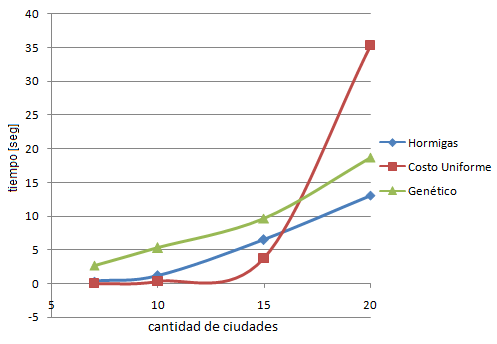
\includegraphics[width=\linewidth]{grafico.png}
\caption{Cantidad de ciudades VS. Tiempo}
\label{fig:cvst}
\end{figure}

A continuación se comparan los porcentajes de aciertos entre el algoritmo de hormigas y genético para 50 iteraciones en una matriz de $7\times7$ (desde Rincón a Esperanza) con $\rho=0.8$ y 7 hormigas. Para el algoritmo genético se establece una población de 8 individuos con 10 generaciones (Tabla \ref{table:tab2}).

\begin{table}[!h]
\begin{center}
\begin{tabular}[c]{ccc} \toprule
Matrices involucradas & Hormigas & Genético\\ \midrule
Distancia       						& 70 & 62 \\
Distancia + Peaje     					& 62 & 58 \\
Distancia + Peaje + Hospedaje   		& 64 & 54 \\
Distancia + Peaje + Hospedaje + Tráfico & 60 & 50 \\ \bottomrule    
\end{tabular}
\end{center}
\caption{Porcentajes de aciertos del camino óptimo en cuanto a las características.}
\label{table:tab2}
\end{table}

Los tiempos de ejecución obtenidos en la tabla \ref{table:tab2} considerando sólo la distancia fueron de $17.03$ segundos y $122.65$ segundos respectivamente.
Cabe aclarar que el resultado real del algoritmo, tanto de hormigas como genético, es aquel camino que mayor ocurrencias tuvo. \\

La tabla \ref{table:tab3} muestra los porcentajes de acierto del camino óptimo variando la cantidad de hormigas, el coeficiente de evaporación y las características involucradas.

\begin{table}[!h]
\begin{center}
\begin{tabular}[c]{ccccc} \toprule
\multirow{2}{*}{Matrices involucradas}
& \multicolumn{2}{c}{7 Hormigas} 
& \multicolumn{2}{c}{14 Hormigas} \\
& $\rho=0.4$ & $\rho=0.8$ & $\rho=0.4$ & $\rho=0.8$ \\  \midrule
D             & 54 & 70 & 72 & 76 \\
D + P         & 62 & 76 & 80 & 88 \\
D + P + H     & 60 & 72 & 74 & 78 \\
D + P + H + T & 64 & 76 & 76 & 82 \\ \bottomrule    
\end{tabular}
\end{center}
\caption{Porcentajes de aciertos del camino óptimo para distintos valores de $N$ y $\rho$.}
\label{table:tab3}
\end{table}

Los tiempos de ejecución para cada combinación de características han sido similares tomando valores aproximados de 18, 71, 36 y 112 segundos respectivamente.

\section{Conclusiones}

El algoritmo de costo uniforme para una representación pequeña obtiene el camino optimo en el menor tiempo pero para una mayor representación se hace cada vez mas pesado y su alcance queda limitado a la potencia del hardware disponible. De todas formas, dada la estructura de las matrices de relación, que no debe recorrer todos los caminos si no sólo donde existe un camino posible, hace que sea una buena opción para la búsqueda del camino óptimo.

El algoritmo genético obtiene el camino optimo en un tiempo intermedio y este no depende del tamaño de la representación. A veces se obtienen caminos con bucles pero eso es algo que puede ser solucionado. 

El algoritmo de hormigas obtiene resultados intermedios pero los tiempos de ejecución no se disparan tanto conforme aumenta la cantidad de ciudades pero esto es relativo a como se establezca la cantidad de hormigas y el coeficiente de evaporación de feromonas. 

Algo común tanto en el algoritmo de hormigas como en el genético es que a medida que incrementa el número de características de evaluación, los porcentajes de acierto del camino óptimo disminuyen. Se puede inferir que demasiada información para determinar un camino hace que los resultados sean peores. Por esto es recomendable no abusar de la cantidad de características y sólo elegir aquellas fundamentales a la hora de determinar la ruta. \\

Una posible mejora para el futuro es cambiar la forma de representación de los datos de entrada. Levantar datos de una base de datos de mapas, o procesar una imagen para detectar nodos y distancias entre ellos.

\begin{thebibliography}{99}
\bibitem{SRAT} %1
Marco Dorigo, Vittorio Maniezzo and Alberto Colorni,
\emph{The Ant System: Optimization by a colony of cooperating agents}. 
IEEE Transactions on Systems, Man, and Cybernetics?Part B, Vol.26, No.1, 1996, pp.1-13.

\bibitem{ID} %2
J. Aguilar, Member IEEE y M. A. Labrador, Senior Member IEEE
\emph{Un algoritmo de enrutamiento distribuido para redes de comunicación basado en sistemas de hormigas}. 
IEEE LATIN AMERICA TRANSACTIONS, VOL. 5, NO. 8,
DECEMBER 2007.
\end{thebibliography}

\end{document}